\documentclass{article}

% if you need to pass options to natbib, use, e.g.:
% \PassOptionsToPackage{numbers, compress}{natbib}
% before loading nips_2016
%
% to avoid loading the natbib package, add option nonatbib:
% \usepackage[nonatbib]{nips_2016}

\usepackage[final]{nips_2016}

% to compile a camera-ready version, add the [final] option, e.g.:
% \usepackage[final]{nips_2016}
\usepackage[utf8]{inputenc} % allow utf-8 input
\usepackage[T1]{fontenc}    % use 8-bit T1 fonts
\usepackage{hyperref}       % hyperlinks
\usepackage{url}            % simple URL typesetting
\usepackage{booktabs}       % professional-quality tables
\usepackage{amsfonts}       % blackboard math symbols
\usepackage{nicefrac}       % compact symbols for 1/2, etc.
\usepackage{microtype}      % microtypography
\usepackage{caption} 
\usepackage{tabularx}
\usepackage{multirow}
\usepackage{graphicx}
\captionsetup[table]{skip=10pt}
\usepackage[flushleft]{threeparttable}
\usepackage{graphicx}
\graphicspath{ {/} }

\usepackage{bbm}
\usepackage{enumitem}
\usepackage[T1]{fontenc} % Use 8-bit encoding that has 256 glyphs
\usepackage{fourier} % Use the Adobe Utopia font for the document - comment this line to return to the LaTeX default
\usepackage[english]{babel} % English language/hyphenation
\usepackage{amsmath,amsfonts,amsthm} % Math packages
\usepackage{amsmath}
\usepackage{lipsum} % Used for inserting dummy 'Lorem ipsum' text into the template
\usepackage[table,xcdraw]{xcolor}
\usepackage{sectsty} % Allows customizing section commands

\title{DOTA2 WIN RATE ESTIMATION VIA DRAFT ANALYSIS}

% The \author macro works with any number of authors. There are two
% commands used to separate the names and addresses of multiple
% authors: \And and \AND.
%
% Using \And between authors leaves it to LaTeX to determine where to
% break the lines. Using \AND forces a line break at that point. So,
% if LaTeX puts 3 of 4 authors names on the first line, and the last
% on the second line, try using \AND instead of \And before the third
% author name.

\author{
  Zhou Fang \\
  Student Number: 1005056467\\
  \texttt{fangzhou@cs.toronto.edu} \\
  \And
  Xiaoshi Huang \\
  Student Number: 995215217\\
  \texttt{xshuang@cs.toronto.edu} \\
  \AND
  Mengxuan Lyu \\
  Student Number: 1005001221\\
  \texttt{shawnlyu@cs.toronto.edu} \\
}

\begin{document}
% \nipsfinalcopy is no longer used

\maketitle

\begin{abstract}
DotA 2 is an esports where 2 teams of 5 players each play against each other. To reach success in this sports category, it is critical to develop a good strategy of picking the avatars, often called heroes or champions. In this project, we compare the performance of most frequently used machine learning algorithms for predicting the match winner from the teams’ drafts in DotA2. Although previous researches attempted this task with simple models, we have made several improvements in our approach aiming to take into account interactions among heroes. We have tested the following machine learning algorithms as the benchmark: Logistic Regression, Naïve Bayesian models, and Support Vector Machines. We also introduced Logistic Regression with hero interactions, Neural Networks and Auto Encoders for this task. Besides, we found the model’s prediction accuracy depends on the player's skill levels where normal level games rely more on the draft than very high level games. 
\end{abstract}

\section{Introduction}
Cybersports, or esports, have had a huge increase in both popularity and attention in recent years. Many different types of analysis have been done on different games, including behaviour analysis, player level ranking, and game mechanism analysis. Among these different topics, one of the most popular is drafting analysis. This involves a game consisting of two or more teams; each team must pick ,or draft, a number of avatars ,often called heroes or champions, depending on the game, from a common pool, and play against each other in the same environment until one team is victorious. Many games ,such as DotA/DotA2, League of Legend, Heroes of the Storms, and \textit{etc}., fall under this category. Due to the existence of synergy and countering between avatars, it is common that after the completion of drafting phase one team will be believed to have a higher win probability than the others. It is in our interest, using machine learning techniques on match records, to understand the mechanism of such win prediction, solely from drafting information. In this research we focus our research using the game DotA2, due to the availability of appropriate datasets, but also because it’s phenomenal championship "The International" in 2011 was at the root of the esports revolution in recent years.

\subsection{DotA 2\cite{Kaggle}}
DotA2 is a computer game in the Multiplayer Online Battle Arena(MOBA) genre. It is played by two teams, called Radiant and Dire which consist of five players each. Each of the players chooses one hero to play with from a pool of heroes in the drafting stage of the game. Each hero has a set of features that define his role in the team and playstyle. Among these features, there are his basic attribute (Strength, Agility or Intelligence) and a unique set of 4 (or for some heroes even more) skills. These features allow each hero to fill several roles in the team, such as "damage dealer" (hero, whose role is to attack the enemies in the fight), "healer" (hero, who mostly heals and otherwise helps his teammates), "caster" (hero, who mostly relies on his spells) etc. 


\subsection{Drafting Phase\cite{grutzik2017predicting}}
In the draft, each team’s captain will take turns banning and picking heroes from a pool. Banning a hero removes it from the pool so neither team can control it; picking one hero would assign its control to a member of the team. As each pick or ban is made, team captains will react and adjust their upcoming draft choices to best suit their own strategy, while simultaneously trying to counter the strategy their opponents appear to be crafting. In total, the draft process takes about 10 minutes, the result of which is both teams now have their 5 hero lineups with which to execute their strategy of destroying the opposing ancient.

\subsection{Project Overview}
Drafting, the process for each team to pick their hero characters, has always been important in the game of Dota 2. Some professional players even claim that 70\% of the game’s outcome depends on the draft. It is in our interest to quantify such influence in the project: draft information (5 heroes on each team, 10 non-repetitive heroes in total) is used to train models to predict the winning team (Radiant/Dire) of the match. More specifically, different machine learning models were trained to predict, based on draft information only, the probability that Radiant will win the game. Assuming there are no draws (which rarely happens in reality), Dire’s win probability will be the complement of Radiant’s value.


\section{Literature review}
A lot of researches have been done in the field of drafting-based win predictions. Among all the papers, we found three papers to be most enlightening to us, in terms of helping us deciding research directions as well as models to approach the question.

\textbf{Performance of Machine Learning Algorithms in Predicting Game Outcome from Drafts in DotA 2\cite{semenov2016performance}}
In this paper, several papers were reviewed, which uses different models to predict game outcome from drafting information. Among the many models used (including random forest, kNN, genetic algorithm, \textit{etc}.) the most popular choice is logistic regression. Drawing from the successes and failures of these attempts, they concluded on two important aspects of draft prediction: 1) a large and consistent dataset should be used for model training and evaluation 2) it is crucial to explore inter- and intra-team hero interactions, such as pair-wise synergy, hero countering, \textit{etc}. Using a large and mechanism-change-free dataset, they trained a Naïve Bayes model and a logistic regression model as the benchmark cases (which are ignorant on hero interactions), and compared models trained using factorization machines and gradient boosting of decision trees to the benchmarks for improvements (shown using AUC of ROC). There is a clear improvement in prediction accuracy, demonstrating the effectiveness of including interactions into the model. 

One deficiency is that both FM and XGBoost models predict less accurately on higher-skilled matches. The author attributed this to high-skilled players being more familiar with most of the heroes and are thus less dependent on drafts. A more natural explanation could be that in higher-skilled games, decisive drafting advantages are less likely to occur due to more experienced players. This could be tested by looking at the differences between the distributions of model predictions on matches of different skill levels.

\textbf{Predicting Outcomes of Professional DotA 2 Matches\cite{grutzik2017predicting}}
Grutzik, \textit{etc}. applied support vector machine (SVM) and neural network (NN) over three major factors that are claimed to be critical to the outcomes: teams that are playing, heroes drafted, and recent performances of players. More specifically, they created a binary indicator to represent the team and player information (1 indicates the corresponding team/player is in-game, 0 otherwise), and constructed a matrix including several features measuring each player’s average performance in 10 immediately preceding games. Results indicated that SVM model outperformed NN model. Player performances held a low correlation with the outcome, while team features lead to overfitting instead of improving performance.

One aspect worth noticing is that the dataset used in this paper ranges from 2011 to 2017, with a total of 47440 games. As the game mechanism had undergone a lot of changes during this period, it implies that the dataset is not consistent itself. This is probably one reason for the underperforming accuracy of their models. As introducing the team feature would result in sparse data, leading to overfitting (especially because the dataset size is relatively small compared to the total team number) and also players’ recent performance does not correlate with the game outcome, we have decided to leave them out of our model, and focus on only draft information.

\textbf{Modelling Game Avatar Synergy and Opposition through Embedding in Multiplayer Online Battle Arena Games\cite{chen2018modeling}}
In this paper, the authors proposed a latent variable model, namely Game Avatar Embedding (GAE), to learn avatar’s numerical representations. GAE models game avatars as vectors in a low-dimensional space learned. They hypothesized that the probability function of a match outcome constitutes of pairwise synergy and opposition interactions formulated by game avatar vectors. Game avatar vectors and other model parameters are learned by gradient descent through maximizing the likelihood function (the winning probabilities) of all observed match outcomes. GAE performance was compared with that of Logistic Regression, Gradient Boosting Decision Tree, Factorization Machine; it was concluded that GAE achieves better classification than other models with 0.7143 accuracy (Same as FM, slightly higher than other models). They also built an ad-hoc baseline method to validate how sensible GAE results to human expert. And they suggested this result can be applied to Hero similarity search and personalized recommendation.

\section{PROBLEM DEFINITION, RESEARCH DESIGN AND METHODS}

\subsection{Problem Definition}
Let the data be a match set $X = \left\{ X _ { 1 } , X _ { 2 } , \dots , X _ { Z } \right\}$ composed of Z matches, with the outcomes of these matches $Y = \left\{ Y _ { 1 } , Y _ { 2 } , \dots , Y _ { Z } \right\} , Y _ { 1 } \in \{ 0,1 \}$ with 1 indicates that $i^{th}$ game ended with Radiant being victorious. Each $X_i$ is a 2N 10-hot vector, with N being the number of unique heroes available in the game:

\begin{center}
$X _ { 1 } [ i ] = \left\{\begin{matrix}
1 & if\ i\leq N\ and\ hero\ i\ was\ in\ radiant\ team \\ 
1 & if\ i> N and\ hero\ i-N\ was\ in\ dire\ team\\ 
0 & otherwise
\end{matrix}\right.$
\end{center}
For model M that takes $X_i$ as input and outputs prediction on the game result $\tilde { Y } _ { i } ^ { M } = M \left( X _ { i } \right) , \tilde { Y } _ { i } \in \{ 0,1 \}$. Define performance of model M as:
\begin{align} 
\begin{split}
  P _ { M } = \operatorname { Pr } \left( \tilde { Y } _ { i } ^ { M } = Y _ { i } \right)
\end{split}         
\end{align}
It is in our interest to investigate the limit of this performance value on different machine learning models.




\subsection{Sources of Data}
The data set used is from the paper by Semenov, \textit{etc}. \cite{semenov2016performance}  Details on the dataset is described as the following: 
"We have collected dataset using Steam API. It contains 5071858 matches from Captains Mode, Random Draft, and Ranked All Pick modes, played between 11th February 2016 10:50:04 GMT and 2nd March 2016 14:07:10 GMT, including skill levels of players. During this period there were no changes to the core mechanics of the game, such as major patches, which makes this dataset especially appropriate for algorithm development and testing. Another key feature of this data is augmenting it with players’ MMR for ranking the games into several brackets depending on the players’ skills."

Recognizing the influence of player levels on the outcome of the games (as investigated by Semenov, \textit{etc}. in their own paper), we have separated the Normal-Skill games (hereby referred to as N games) and Very-High-Skill games (VH games) into two datasets. Some more robust models (such as benchmarks and improvements on the benchmark models) were tested on the overall dataset (due to time constraint), while the more sensitive non-linear models were trained and tested on N/VH data sets separately, with some occasional cross-checking between the data sets.
Due to the transitional nature of High-Skill games between N games and VH games, performances of models applied to this batch of games is expected to lie within their respective performances on N games and VH games. This batch of data is therefore omitted during testing, mainly for saving project time. 



\subsection{Research Design}
Several types of models were experimented on the data sets, to see which ones produce the best prediction performances. They are categorized as the following genres.

\subsubsection{Benchmark Models: generalized linear methods}
Three classical models were chosen as the benchmark models: Naïve Bayesian models, logistic regression models, and Support Vector Machines. They were chosen because of their robustness in performances, as well as the ability to directly take many forms of inputs with very little pre-processing required. Performances of these models serve as a standard against which other models are compared.

\subsubsection{Improvement on Benchmark Models}
Several machine learning techniques are applied to the benchmark models, trying to improve their performances:

a). Adaboost: Adaboost was applied, using the benchmark Naïve Bayesian model as the base learner. The idea was that via adaboost, it would be possible to force the Naïve Bayesian model to focus on the more difficulty match sets, thus increasing prediction accuracy.
    
b). Principle Component Analysis (PCA): benchmark models were applied to not the raw match drafting vectors, but a portion of the top Principle Components of the drafting vectors. More specifically, benchmark models were applied to the first 70 principal components, in the hope that: \textbf{\textit{i)}} robustness would be increase. \textbf{\textit{ii)}} focusing on key information could possibly increase prediction accuracy.
    
c). Logistic Regression with Synergy and Countering (LRSC): by their formulations, all three benchmark model consider the only comparison of single hero strengths. Since it is commonly known that interactions between heroes, within or across teams, have decisive influences on the games’ outcomes, it is natural to expand the basic logistic regression model to incorporate such interactions into the model (it is not as convenient to do similar model expansions with SVM and Naïve Bayesian models). The idea is very similar to the Synergy Matrix and Opposition Matrix of the GAE model proposed in Chen’s paper\cite{chen2018modeling}:
    Instead of proposing that the game result is characterized by 
    \begin{align} 
    \begin{split}
      \operatorname { Pr } \left( Y _ { i } = 1 \right) \propto \frac { 1 } { 1 + \exp \left( w ^ { T } X _ { i } \right) }
    \end{split}         
    \end{align}
    For some 2Nx1 weight vector w, the proposal is that there exists some NxN matrix S (for synergy) and C (for countering) between every hero-pair, and that the probability for team radiant to win the game is modified as follows:
    \begin{align} 
    \begin{split}
      \operatorname { Pr } \left( Y _ { i } = 1 \right) \propto \frac { 1 } { 1 + \exp \left( X _ { r , i } ^ { T } S X _ { r , i } - X _ { d , i } ^ { T } S X _ { d , i } + X _ { r , i } ^ { T } C X _ { d , i } \right) }
    \end{split}         
    \end{align}

In which $X_{r,i},X_{d,i}$ are both Nx1, 5 hot binary vectors representing the draft composition of team radiant and team dire, respectively. By definition, $[X_{r,i},X_{d,i} ]= X_i$


\subsubsection{Non-Linear Models: Neural Networks}
Because information contained in the draft composition is likely to be non-linear, it is decided to also try with neural networks of different structures, as a non-linear method of extracting such information. Both fully connected neural networks, as well as neural networks with some internal structures, meant to mimic Dota 2’s game mechanics and help the network to understand the game, are implemented.

\subsubsection{Combining Neural Networks with Classical Models: Auto Encoders}
Following the same argument as above, it is very likely that PCA on the draft vectors would not be able to successfully extract all of the information contained. But dimensionality reduction techniques does come with a few desirable effects, such as more compact notations as well as easier interpretability. This is the motivation to use Auto Encoders to replace PCA in the "improvement to benchmark" section, as a non-linear dimension reduction technique. Generalized linear methods, such as logistic regression and LRSC, were apply to the encoded data for modeling. Due to server memory constraints, certain larger models (such as LRSC-on-encoding) were only trained and tested using part of the data.





\section{RESULTS AND DISCUSSION}
\subsection{Benchmark Models: generalized linear methods}




Several observations of Table \ref{table:benchmark} can be made here:

a). In general, all three benchmark models work equally well on all three sets of data; among the three, logistic regression models show a little bit more robustness.

b). All models produce much better estimates than random guess based on data sets’ inherent biases.

c). The difference in predictability between N games and VH games is only amplified under model prediction powers. For a more detailed discussion on this phenomenon, refer to Appendix 2: Why are Normal-Skilled Games Easier to Predict?

\subsection{Improvement on Benchmark Models}



Several observations of Table \ref{table:improved_benchmark} can be made here:

a). Adaboost seems to be quickly converging to a threshold accuracy, which is only slightly better than the single Naïve Bayesian model.


b). It is clear that performing PCA on the dataset and applying benchmark models on the principal components did not improve the prediction performance. This is understandable since the main idea behind PCA is linear dimensional reduction; any information that can be stored in the principal components would have already been extracted by the benchmark models from the original draft vectors. The main advantage of PCA is to offer robustness and prevent overfitting, but in this case, there is no overfitting to start with, thanks to the enormous amount of data present in both N game and VH game data sets.


c). LRSC clearly offers the best improvement here, not only superior to the other two improvements but also exceeding the performance of all three benchmark models by a significant amount on N games. The reason is that LRSC is not a linear modification of the benchmark models; it improves on logistic regression model in a non-linear that not only expand the model capacity by a factor of N (the number of heroes in the game) but also incorporates some understanding on the game mechanics. More specifically, LRSC allows the model to describe the interaction between heroes, an aspect that is clearly influencing the game but is lacking in all benchmark models.

From these improvements on the benchmark models (especially LRSC, since it produces the most increase in prediction accuracy), some preliminary conclusions can be drawn:
\begin{enumerate}
    \item Hero interactions are decisive to game outcome prediction.
    \item Game-outcome influencing information in the draft, excluding those already extracted by the benchmark models, is most likely non-linear in nature.
\end{enumerate}

\subsection{Non-Linear Models: Fully Connected Neural Networks}

\begin{figure}[htb]
\begin{minipage}[t]{0.5\linewidth}
\centering
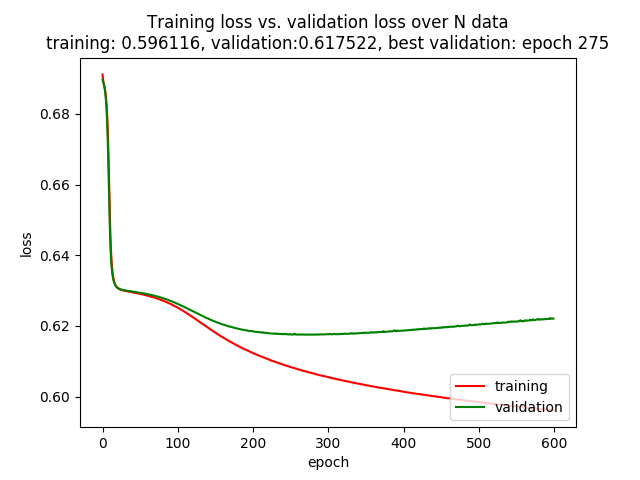
\includegraphics[width=3.0in]{N_loss.png}
\end{minipage}%
\begin{minipage}[t]{0.5\linewidth}
\centering
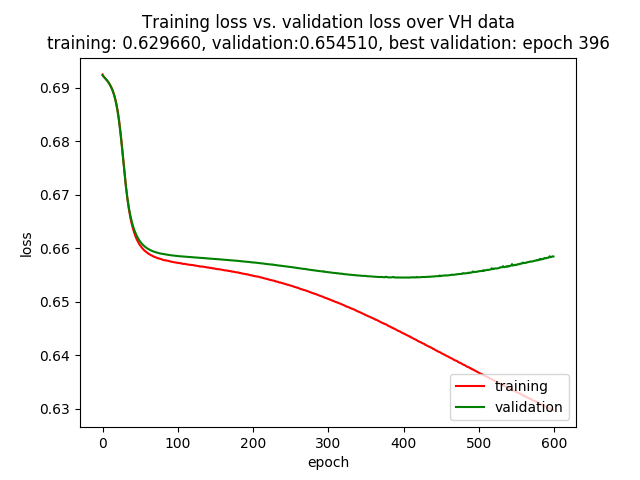
\includegraphics[width=3.0in]{VH_loss.png}
\end{minipage}
\caption{Training and Validation loss of FCNN with layers: 226-160-100-1 }
\label{image:FCC}
\end{figure}

As described in Table \ref{table:FCC}, fully connected neural networks, consisted of a different number of layers and nodes, demonstrated good predictive power on both data sets. The best score on N game data set is only slightly inferior to the LRSC result, while the best performance on VH game data set improves LRSC’s accuracy by more than 2\%. Figure \ref{image:FCC} shows the training loss and validation loss of the best FCC model on N and VH game dataset separately. Refer to the next section for more discussion about experiment results with fully connected neural networks.


\subsection{Non-Linear Models: Structured Neural Networks}
The structured neural networks can be illustrated using Figure \ref{image:pic1}.

% \begin{figure}
%  \centering 
%  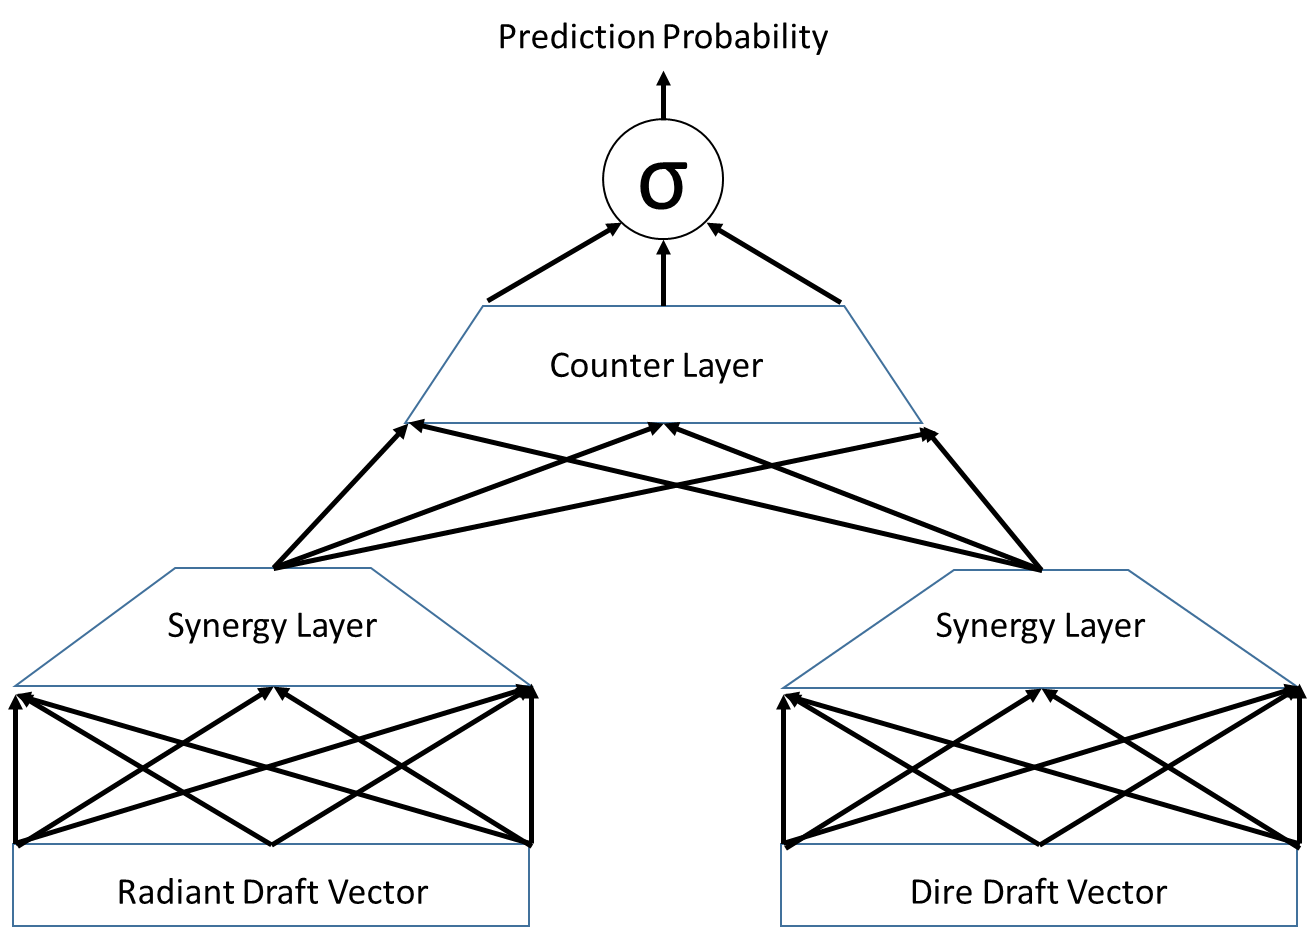
\includegraphics[scale=0.6]{Picture1.png}
%  \caption{Illustration on Structured Neural Network Architecture}
%  \label{image:pic1}
% \end{figure}

\begin{figure}[htb]
\begin{minipage}[t]{0.5\linewidth}
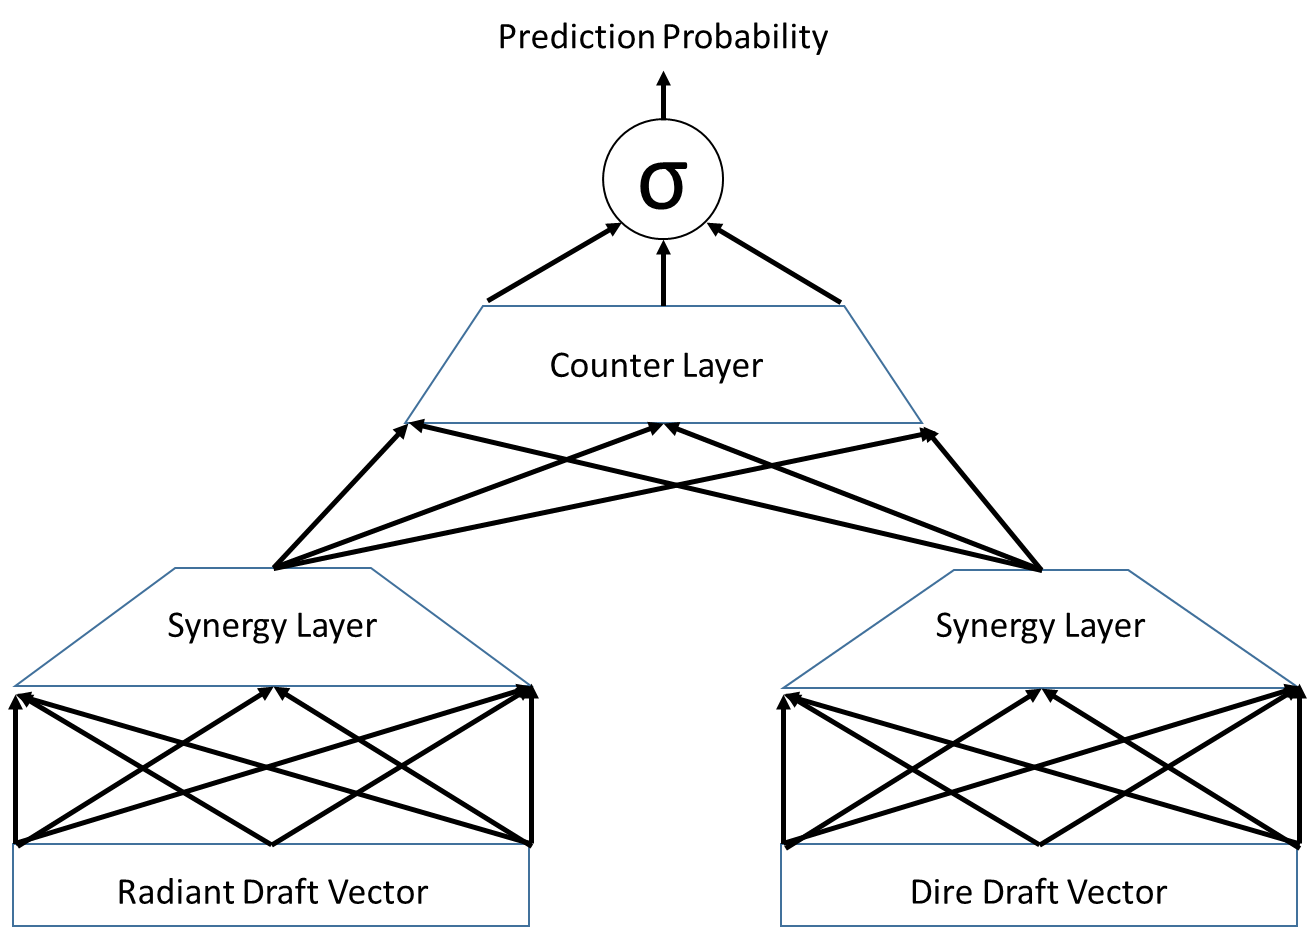
\includegraphics[width=2.4in]{Picture1.png}
\caption{Illustration on Structured \\ Neural Network Architecture}
\label{image:pic1}
\end{minipage}%
\begin{minipage}[t]{0.5\linewidth}
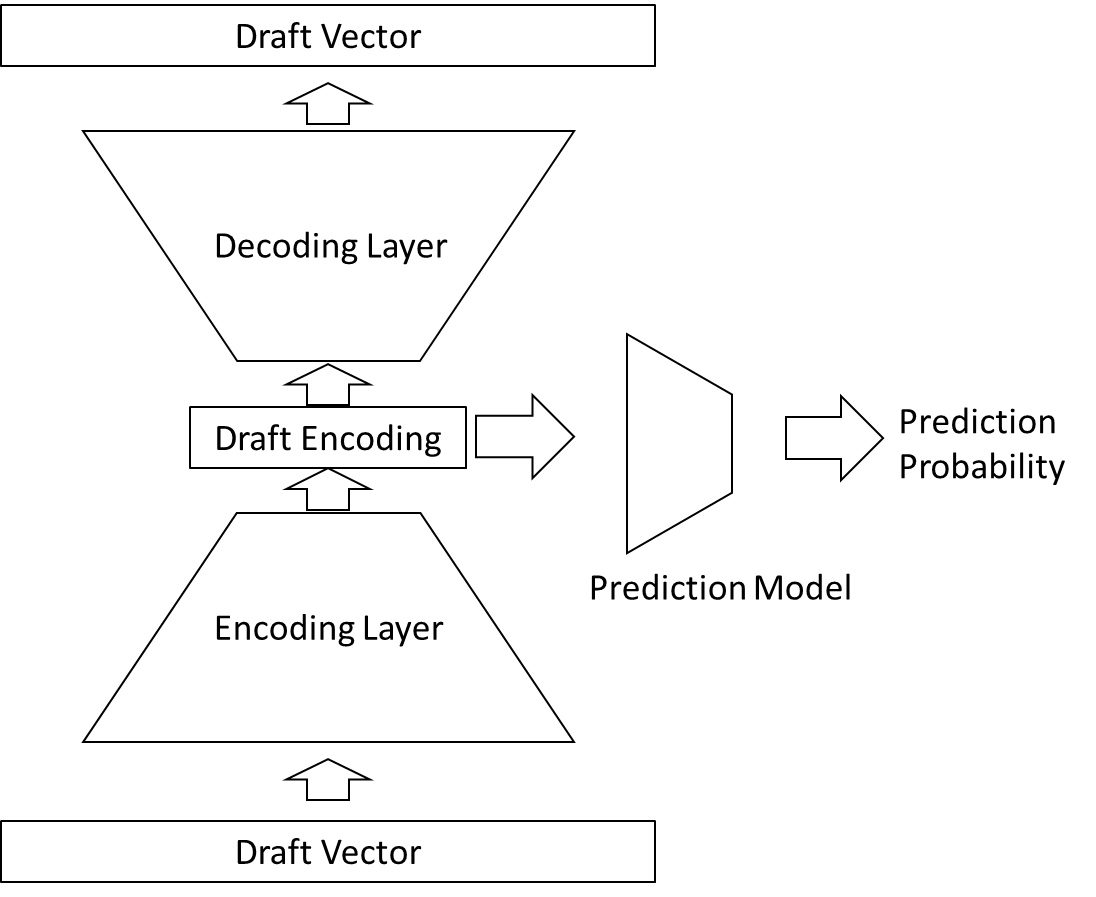
\includegraphics[width=2.4in]{Picture2.png}
\caption{Illustration on Using Auto Encoder for Game Outcome Prediction}
\label{image:pic2}
\end{minipage}
\end{figure}


Each team’s draft vector is first passed through the same Synergy Layer, a fully connected neural network that is should work out the interaction between heroes within teams. The outputs of Synergy Layers are then passed to a Counter Layer, a fully connected neural network that is supposed to compare two team compositions, then to a sigmoid node that calculates the win probability. The detailed structures experimented, as well as their prediction accuracies on the test sets, were shown in Table \ref{table:FC_Synergy_Counter}.

Combining Table \ref{table:FC_Synergy_Counter} with results presented in Table \ref{table:FCC}, a few interesting observations can be made:

a). Dropout: the use of dropout in both cases did not help much. This can be attributed to the size of training sets. Dropouts are mainly used as a tool to prevent model overfitting, which was never a problem in this project since the sheer size of training data itself prevents most of the overfitting behaviour.

b). N Games: both models work pretty well on N game data set, approaching the optimal prediction accuracy obtained from LRSC on draft vectors. This seems to be suggesting that it is possible for 66\% prediction accuracy to be close to the optimal accuracy models can achieve on N games.

c). VH Games: both structured neural networks and LRSC fails in comparison to fully connected neural networks when it comes down to predicting VH games: 61\% vs. 62.3\%, a significant gap in this project. The implication of this result is very interesting: it seems to suggest that the information hidden in VH game draft compositions is not only non-linear but cannot be simply viewed and analyzed from an intra-team and inter-team perspective. The reason behind this conjecture is that both LRSC and structured neural networks are designed to considered two teams separately, then together (via Synergy and Countering matrices in LRSC, and Synergy and Counter layers in structured neural nets); fully connected neural nets do not have this constraint. By achieving a much higher prediction accuracy on VH games using fully connected neural nets, it seems to suggest that such division of draft information is not the best approach, at least not with VH game predictions.

d). The upper limit in prediction accuracy: Even though there is no clear evidence, it is suspected that the ~66\% prediction accuracy achieve by LRSC and fully connected neural network models on N game data set might be approaching the upper limits of similar estimation tasks in Dota 2, given draft information only. This claim is supported by the fact that several different models, with vastly different structures, seem to be approaching the same threshold value. An estimate on the higher bound of accuracy would be around 68\%-70\%. Even though this value might be low at first appearance, it is reasonable considering the fact that unlike tasks such as image recognition, Dota 2 match outcomes are inherently stochastic: game progression are prone to human errors, therefore drafts could only set a bulk probability for the outcome. 


\subsection{Combining Neural Networks with Classical Models: Auto Encoders}


The concept of using Auto Encoder for game outcome predictions can be described in Figure \ref{image:pic2}.

As stated before, the key concept is to replace PCA with a non-linear Auto Encoder to compress draft vectors, then train models using these draft encodings, instead of the draft vectors. The hope is that by pre-processing the draft vectors, the non-linear content would be extracted into the encodings and be available to models (such as Logistic Regressions and LRSC) that otherwise would not have access to such information.




From table \ref{table:autoencoder_prediction}, it can be observed that Auto Encoders, combined with either logistic regression or LRSC models, do not offer improvement in prediction accuracy. Clearly, the extraction of important information influencing game results, which is the intention of such structure, did not happen, while the information lost during compression decreased prediction accuracies. 
One possible explanation for the failure of extracting information into the encoding is that the Auto Encoder structure doesn’t care, or even know, about the game outcome; as a result, it reconstructs the draft very well, but the encoding offers little help to predicting game outcomes. One way to improve on this idea is to modify the structure to force the game outcome into the encoding: by aiming the Auto Encoder at not only reconstructing the draft vector but also the game result. This would change the structure into a combination of Auto Encoders and outcome-aimed neural networks. Due to project time limitation, this idea is not implemented.

\subsection{Conclusion}
Several different types of machine learning models have been implemented, aimed at using the draft vectors from Dota 2 matches to predict the game outcomes. Due to the impact of player skill level differences on the games, data sets have been divided into Normal-Skilled games and Very-High-Skilled games, according to players’ MMR ratings. Models were trained and tested on the two datasets separately.
LRSC model achieved a prediction accuracy of 65.88\% on the N game testing set, with fully connected neural network following with 65.6\%. On VH games, which are harder to predict due to higher player skill levels, fully connected neural network achieved 62.35\% prediction accuracy on the test set with a two hidden layer structure (160-100). Both results were below our initial expectations on prediction accuracy (we were hoping for 70\% before project commencement), but they are acceptable considering the stochastic nature of Dota 2 game outcomes.
It is suspected that on N game dataset, both LRSC and neural network models might be approaching the accuracy upper limits in similar estimation tasks, due to the high Bayesian error in such data sets. On VH data set, there still seems to be more information not yet extracted from the draft vectors.

\subsection{Limitations and Future Work}
Due to the constraint in time and computation resources, several ideas on either improving the model performances or different model structures were not implemented. A few examples are listed below:
\begin{enumerate}
    \item
    Hyper-parameters in neural network structures can be tuned more carefully. Alternatively, they can be determined via a Gaussian Process.
    \item
    As discussed in the Auto Encoder section, a semi-auto encoder could be built to force some of the game outcome information into the encoding. 
    \item
    Current models are based only on draft information. A slightly different perspective on this topic would be to consider not only the drafts, but game progression information as well, and build models for live prediction of win probabilities. Successful implementation of this type is Valve’s Dota Plus, a tool that is recognized to be very helpful in understanding the game among audiences as well as professional players.
\end{enumerate}

 \renewcommand{\thefootnote}{}
\footnotetext{source code could be found via \href{https://github.com/risingdhxs/CSC2515Dota2DraftPredictionProject}{CSC2515Dota2DraftPredictionProject.git}.}


\bibliographystyle{plain}
\bibliography{csc2515}

\newpage
\begin{appendix}
\section*{Appendices}
\subsection*{Appendix 1: Result tables}


\bgroup
\def\arraystretch{1.7}%  1 is the default, change whatever you need
{
\begin{table}[htb]
\centering
\begin{tabularx}{\textwidth}{ |X|l|l|l| } 
\hline
\textbf{Models} & \textbf{All Matches} & \textbf{N Games} & \textbf{VH Games} \\
\hline
Inherent Bias & 53.27\% & 54.02\% & 52.11\% \\
\hline
Naïve Bayes & 62.21\%/62.12\% & 64.25\%/64.18\% & 60.70\%/60.50\% \\
\hline
Logistic Regression & 62.66\%/62.63\% & 64.39\%/64.42\% & 60.70\%/60.50\% \\
\hline
Linear SVM & 62.66\%/62.13\% & 64.26\%/64.25\% & 60.60\%/60.40\% \\

\hline
\end{tabularx}
\caption{Training/Testing Accuracies for Benchmark Models}
\label{table:benchmark}
\end{table}}
\egroup







\bgroup
\def\arraystretch{1.7}%  1 is the default, change whatever you need
{
\begin{table}[htb]
\begin{threeparttable}
\centering
\begin{tabularx}{\textwidth}{ |X|l|l|l| } 
\hline
\textbf{Models} & \textbf{All Matches} & \textbf{N Games} & \textbf{VH Games} \\
\hline
Adaboost on Naïve Bayesian & 61\%  & N/A*  & N/A* \\
\hline
LRSC & 65.10\%/64.13\% & 67.30\%/65.88\% & 65.32\%/60.97\% \\
\hline
Naïve Bayes on PC 70 & 59.82\%/59.73\% & 61.58\%/61.55\% & N/A** \\
\hline
Logistic Regression on PC 70 & 60.10\%/60.02\% & 62.21\%/62.24\% & N/A** \\
\hline
\end{tabularx}
       \begin{tablenotes}
            \item[*]  Adaboost on Naïve Bayesian were only tested on All Matches.
            \item[**] Naïve Bayesian on PC 70 and Logistic Regression on PC 70 were not tested on VH game sets, because it is clear from the other two sets that they would not produce any significant increase in performance.
        \end{tablenotes}
     \end{threeparttable}
\caption{Training/Testing Accuracies for Improved Benchmark Models}
\label{table:improved_benchmark}
\end{table}}
\egroup





\bgroup
\def\arraystretch{1.7}%  1 is the default, change whatever you need
{
\begin{table}[htb]
\centering
\begin{tabularx}{\textwidth}{ |X|l|l|l|l|l|l|l| } 
\hline

\textbf{Hidden Layer}& & \multicolumn{3}{c|}{\textbf{N Games}} & \multicolumn{3}{c|}{\textbf{VH Games}} \\\cline{3-8}

\textbf{Node Number} & \textbf{Dropout?} & \textbf{Train} & \textbf{Valid} & \textbf{Test}  & \textbf{Train} & \textbf{Valid} & \textbf{Test}\\
\hline
100 & False & 65.37\% & 65.17\% & 65.17\% & 61.02\% & 60.77\% & 61.98\% \\
\hline
100 & True & 64.76\% & 64.66\% & 64.60\% & 60.63\% & 60.43\% & 61.39\% \\
\hline
160-100 & False & 67.84\% & 65.69\% & \textbf{65.58\%} & 64.46\% & 61.25\% & \textbf{62.35\%} \\
\hline
160-100 & True & 65.93\% & 65.13\% & 65.03\% & 61.39\% & 60.75\% & 61.74\% \\
\hline
160-100-20 & False & 68.44\% & 65.60\% & 65.61\% & 66.73\% & 61.07\% & 62.25\% \\
\hline
160-100-20 & True & 66.04\% & 65.03\% & 64.97\% & 61.45\% & 60.74\% & 61.85\% \\
\hline
10 & False & 64.69\% & 64.64\% & 64.64\% & 60.76\% & 60.72\% & 61.86\% \\
\hline
10 & True & 64.25\% & 64.18\% & 64.13\% & 60.07\% & 59.92\% & 61.05\% \\
\hline
160-10 & False & 67.76\% & 65.66\% & 65.62\% & 64.25\% & 61.07\% & 62.24\% \\
\hline
160-10 & True & 64.97\% & 64.43\% & 64.32\% & 60.91\% & 60.39\% & 61.61\% \\
\hline
160-100-100 & False & 68.41\% & 65.60\% & 65.61\% & 66.98\% & 61.07\% & 62.22\% \\
\hline
160-100-100 & True & 66.19\% & 65.10\% & 65.01\% & 61.71\% & 60.83\% & 61.83\% \\
\hline
\end{tabularx}
\caption{Fully Connected Neural Network Performances}
\label{table:FCC}
\end{table}}
\egroup


\bgroup
\def\arraystretch{1.7}%  1 is the default, change whatever you need
{
\begin{table}[htb]
\centering
\begin{tabularx}{\textwidth}{ |X|l|l|l|l|l|l|l| } 
\hline
\textbf{Synergy Layer Node Number}    & \textbf{Counter Layer Node Number}     & \textbf{Dropout} & \textbf{N Games} & \textbf{VH
Games} \\ \hline
\multirow{2}{*}{100-100}     & \multirow{2}{*}{200-100-50}   & True    & 65.1\%                                            & 60.76\%                                            \\ \cline{3-5} 
                             &                               & False   & 65.24\%                                           & 60.78\%                                            \\ \hline
\multirow{2}{*}{100-100-100} & \multirow{2}{*}{200-10-50-25} & True    & 64.75\%                                           & 60.69\%                                            \\ \cline{3-5} 
                             &                               & False   & 64.92\%                                           & 60.81\%                                            \\ \hline
\multirow{2}{*}{500-200}     & \multirow{2}{*}{400-100-50}   & True    & 64.88\%                                           & 60.77\%                                            \\ \cline{3-5} 
                             &                               & False   & 64.93\%                                           & 60.82\%                                            \\ \hline
\multirow{2}{*}{1000-250}    & \multirow{2}{*}{500-100}      & True    & 64.96\%                                           & 60.84\%                                            \\ \cline{3-5} 
                             &                               & False   & 64.9\%                                            & 60.84\%                                            \\ \hline
50-50                        & 100-50                        & False   & 65.14\%                                           & 60.93\%                                            \\ \hline
\end{tabularx}
\caption{Structured Neural Networks Prediction Accuracy on Test Set}
\label{table:FC_Synergy_Counter}
\end{table}}
\egroup

\bgroup
\def\arraystretch{1.7}%  1 is the default, change whatever you need
{
\begin{table}
\begin{threeparttable}
\centering
\begin{tabularx}{\textwidth}{|X|l|l|l|l|l|l|l|}
\hline
\textbf{Encoder Node}& \textbf{Decoding} & \multicolumn{3}{c|}{\textbf{N Games}} & \multicolumn{3}{c|}{\textbf{VH Games}} \\\cline{3-8}

\textbf{Number} & \textbf{Method} & \textbf{Train} & \textbf{Valid} & \textbf{Test}  & \textbf{Train} & \textbf{Valid} & \textbf{Test}\\
\hline
\multirow{2}{*}{100-75-50}                                                         & LR                                                                         & 59.19\%  & 59.27\% & 59.23\% & 58.17\%  & 58.03\%  & 58.0\%  \\ \cline{2-8} 
& LRSC                                                                       &          &         &         &     61.21\%     &     59.09\%     &    59.01\%     \\ \hline
\multirow{2}{*}{110-90-70}                                                         & LR                                                                         & 59.51\%  & 59.46\% & 59.51\% & 58.53\%  & 58.33\%  & 58.4\%  \\ \cline{2-8} 
                                                                                   & LRSC                                                                       &          &         &         &     62.93\%     &   58.5\%       &   58.44\%      \\ \hline
\multirow{2}{*}{110-90-80-70}                                                         & LR                                                                         & 59.5\%  & 59.56\% & 59.48\% & 57.09\%  & 56.96\%  & 56.99\%  \\ \cline{2-8} 
                                                                                   & LRSC                                                                       &          &         &         &      60.17\%    &    57.57\%      &   57.37\%      \\ \hline
\multirow{2}{*}{120-150-120-90}                                                    & LR                                                                         &     60.61\%     &   60.58\%      &    60.62\%     & 58.17\%  & 58.04\%  & 57.99\% \\ \cline{2-8} 
                                                                                   & LRSC                                                                       &          &         &         &    64.65\%      &   57.81\%       &    57.75\%     \\ \hline
\multirow{2}{*}{130-150-180*}                                                      & LR                                                                         & 61.22\%  & 61.24\% & 61.16\% & 56.8\%   & 56.64\%  & 56.78\% \\ \cline{2-8} 
                                                                                   & LRSC                                                                       &          &         &         & 88.18\%  & 53.94\%  & 52.76\% \\ \hline
\multirow{2}{*}{\begin{tabular}[c]{@{}l@{}}130-160-200-\\ 160-120-90\end{tabular}} & LR                                                                         & 58.07\%  & 58.04\% & 58.04\% & 56.8\%   & 56.64\%  & 56.78\% \\ \cline{2-8} 
                                                                                   & LRSC                                                                       &          &         &         &   61.8\%       &   56.59\%       &    56.78\%     \\ \hline


\end{tabularx}
       \begin{tablenotes}
            \item[*]  Due to size of encoding vector, it is necessary to discard a large portion of the training data due to server memory constraint. This leads to severe overfitting of LRSC models
        \end{tablenotes}
     \end{threeparttable}
\caption{Auto Encoder Prediction Accuracies, Using Logistic Regression and LRSC Model}
\label{table:autoencoder_prediction}
\end{table}}
\egroup

\newpage
\subsection*{Appendix 2: Why are Normal-Skilled Games Easier to Predict?}
The difference between the predictability of N games and VH games have already been noticed before.\cite{chen2018modeling} There are two intuitively plausible explanations for such phenomenon: 

a) it is easier to draft more decisive team compositions in N games (due to player inexperience), which leads to easier predictions 

b) team compositions are similar in both N and VH games, but lack in player skills leads to certain team compositions, fair in VH games, more imbalanced in N games. It is possible to investigate these two hypothesis by applying models, with the same structure but different training data, on the same set of testing data and observe the distribution of game result probabilities. Here we choose two logistic regression models, trained on the training sets of N and VH games, and make game result probability estimates on the respective test data set.


\begin{figure}[htb]
 \centering 
 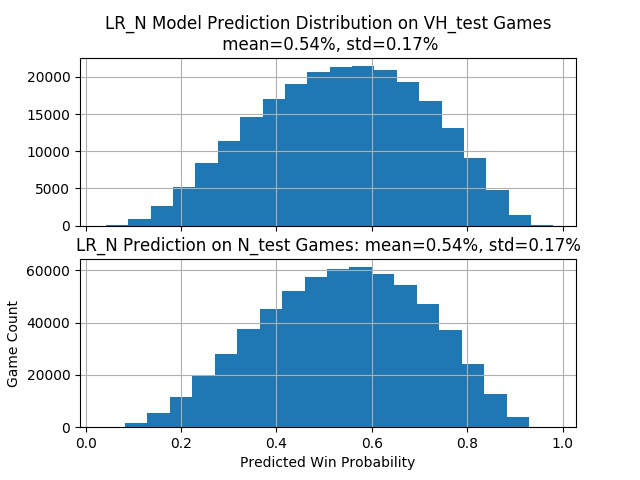
\includegraphics[scale=0.8]{Picture3.png}
 \caption{N-Game LR Model Prediction Probability on Test Sets}
 \label{image:pic3}
\end{figure}


\begin{figure}[htb]
 \centering 
 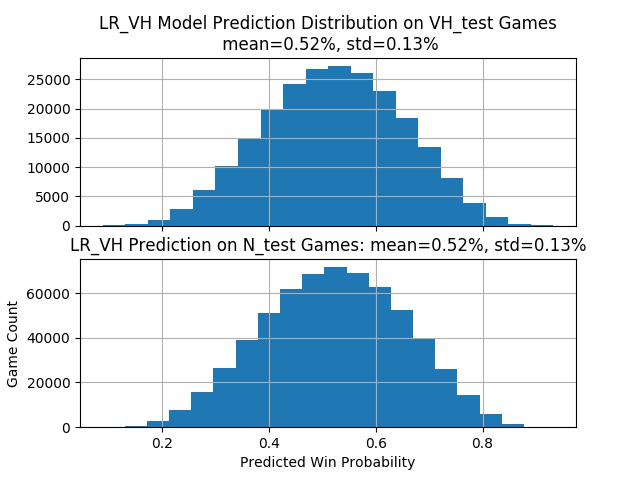
\includegraphics[scale=0.8]{Picture4.png}
 \caption{VH-Game LR Model Prediction Probability on Test Sets}
 \label{image:pic4}
\end{figure}


\begin{figure}[htb]
 \centering 
 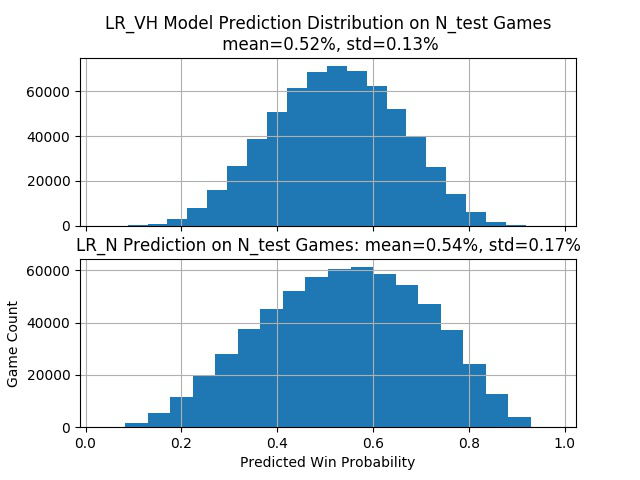
\includegraphics[scale=0.8]{Picture5.png}
 \caption{N and VH LR Model Prediction Probability on N-Game Test Sets}
 \label{image:pic5}
\end{figure}
From these three figures, it is clear that the difference is not caused by drafts, but by player skills. When a single LR model (whether trained using N game data or VH game data) is used to estimate both test sets, the prediction distributions are always the same. But when two different models were used to make predictions on the same data set, N-game model tends to make more deterministic predictions (indicated by a higher standard deviation). This can only mean that certain drafts, while being considered fair in VH games, are evaluated to be more imbalanced in N games, either in a good way or a bad way. Certainly this is caused by the difference in player skill level, such as (but not limited to) hero pool size, game understanding, countering opponent heroes via lane change or gear choices, etc.

\end{appendix}

\end{document}
